\documentclass{article}
\usepackage{tikz}
\usepackage{amsmath}
\usetikzlibrary{arrows.meta, calc, patterns, decorations.pathreplacing, positioning}
\usepackage[paperwidth=36cm,paperheight=25cm,margin=0.3cm]{geometry}
\pagestyle{empty}

\begin{document}
\centering
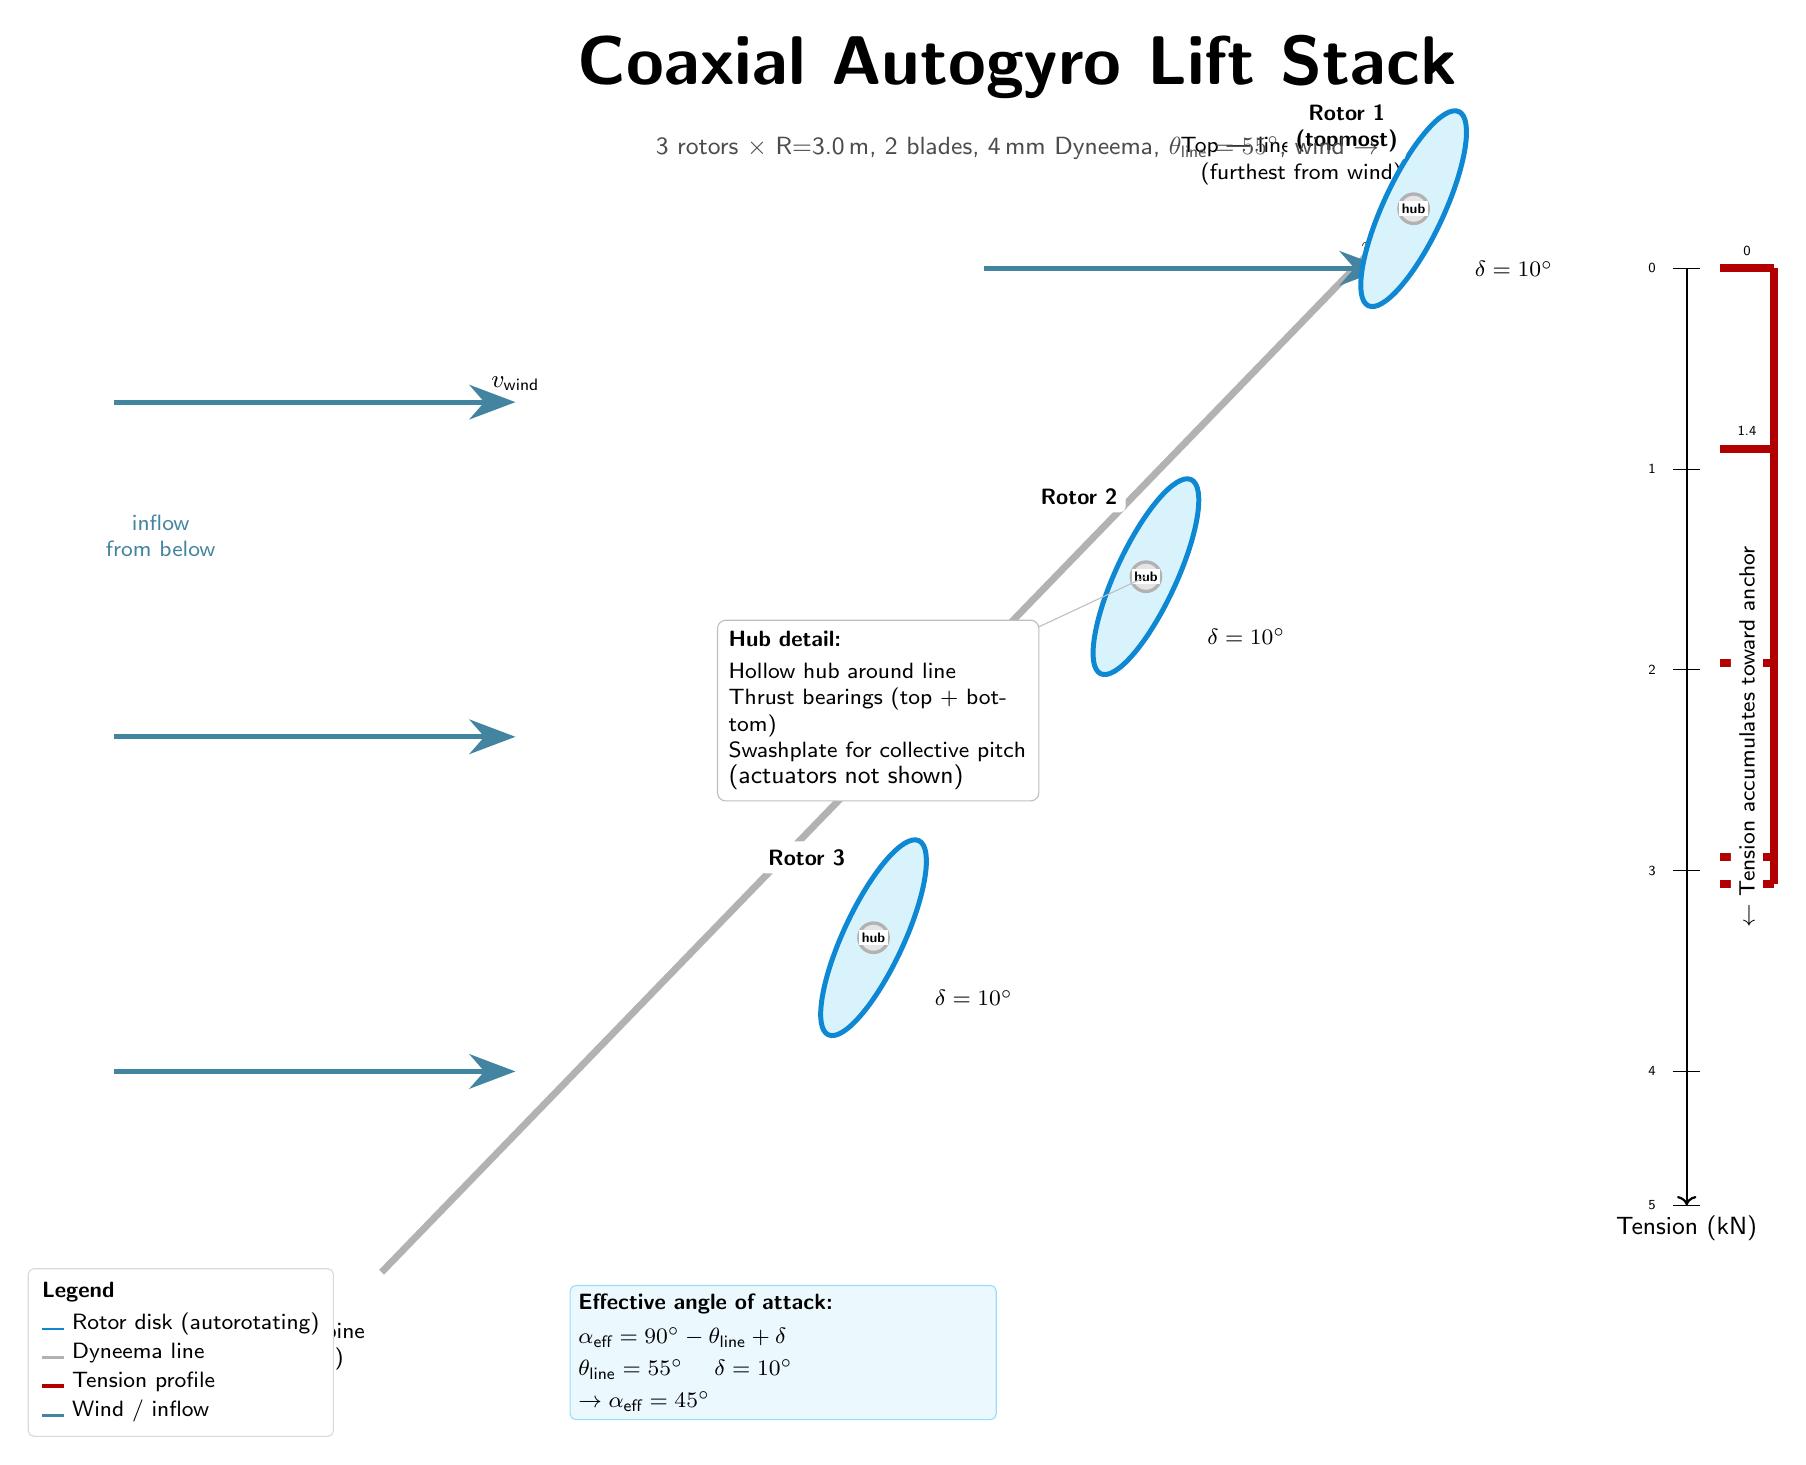
\begin{tikzpicture}[scale=0.85,
  line/.style={draw=gray!60, line width=2.5pt},
  disk/.style={draw=cyan!70!blue, fill=cyan!15, line width=1.8pt},
  hub/.style={draw=gray!60, fill=gray!20, line width=1.2pt},
  tensionline/.style={draw=red!70!black, line width=2.8pt},
  annot/.style={font=\footnotesize\sffamily, fill=white, inner sep=3pt, rounded corners=2pt},
  windarrow/.style={-{Stealth[scale=1.5]}, draw=cyan!60!black, line width=1.8pt},
]

% Wind L->R, anchor upwind (left), kites trail downwind (right)
\coordinate (anchor) at (-6.0, -7.0);
\coordinate (r3)     at (1.5, -1.9);
\coordinate (r2)     at (5.5, 3.5);
\coordinate (top)    at (9.5, 9.0);

\draw[line] (anchor) -- (top);
\node[annot, above left=0.1cm and 0.1cm of top, align=right] {Top --- line terminates\\ (furthest from wind)};
\node[annot, below left=0.2cm and 0.1cm of anchor, align=left] {Anchor\\ to Kite Turbine\\ (upwind end)};

\draw[windarrow] (-10, 6) -- (-4, 6) node[above, font=\small\sffamily] {$v_\text{wind}$};
\draw[windarrow] (-10, 1) -- (-4, 1);
\draw[windarrow] (-10, -4) -- (-4, -4);
\draw[windarrow] (3, 8) -- (9, 8) node[above, font=\small\sffamily] {$v_\text{wind}$};

\node[font=\footnotesize\sffamily, text=cyan!60!black, align=center] at (-9.3, 4.0) {inflow\\ from below};

% Rotor 1 -- centred on line, top edge tilts TOWARD wind (left)
% Line at ~55 deg. Disk perpendicular-to-line = ellipse major axis at 55 deg.
% Tilt delta=10 deg toward wind = rotate CCW by 10 deg = major axis at 65 deg.
\coordinate (h1) at ($(top)!0.02!(r2)$);
\draw[disk, rotate around={65:(h1)}] (h1) ellipse (1.6 and 0.45);
\draw[hub] (h1) circle (0.22);
\node[font=\tiny\sffamily\bfseries, fill=white, inner sep=1pt] at (h1) {hub};
\node[annot, font=\footnotesize\sffamily\bfseries, align=center] at ($(h1) + (-1.0, 1.2)$) {Rotor 1\\(topmost)};
\node[annot, font=\footnotesize\sffamily] at ($(h1) + (1.5, -0.9)$) {$\delta=10^\circ$};

% Rotor 2
\coordinate (h2) at ($(r2)!0.02!(r3)$);
\draw[disk, rotate around={65:(h2)}] (h2) ellipse (1.6 and 0.45);
\draw[hub] (h2) circle (0.22);
\node[font=\tiny\sffamily\bfseries, fill=white, inner sep=1pt] at (h2) {hub};
\node[annot, font=\footnotesize\sffamily\bfseries] at ($(h2) + (-1.0, 1.2)$) {Rotor 2};
\node[annot, font=\footnotesize\sffamily] at ($(h2) + (1.5, -0.9)$) {$\delta=10^\circ$};

% Rotor 3
\coordinate (h3) at ($(r3)!0.02!(anchor)$);
\draw[disk, rotate around={65:(h3)}] (h3) ellipse (1.6 and 0.45);
\draw[hub] (h3) circle (0.22);
\node[font=\tiny\sffamily\bfseries, fill=white, inner sep=1pt] at (h3) {hub};
\node[annot, font=\footnotesize\sffamily\bfseries] at ($(h3) + (-1.0, 1.2)$) {Rotor 3};
\node[annot, font=\footnotesize\sffamily] at ($(h3) + (1.5, -0.9)$) {$\delta=10^\circ$};

% Tension axis
\coordinate (taxis_top) at (13.5, 8.0);
\coordinate (taxis_bot) at (13.5, -6.0);
\draw[thick, ->] (taxis_top) -- (taxis_bot) node[below, font=\small\sffamily] {Tension (kN)};

\foreach \y/\val in {8.0/0, 5.0/1, 2.0/2, -1.0/3, -4.0/4, -6.0/5} {
    \draw (13.3, \y) -- (13.7, \y);
    \node[font=\tiny\sffamily, left=0.1cm] at (13.3, \y) {\val};
}

\draw[tensionline] (14.0, 8.0) -- node[above, font=\tiny\sffamily] {0} (14.8, 8.0);
\draw[tensionline] (14.8, 8.0) -- (14.8, 5.3);
\draw[tensionline] (14.0, 5.3) -- node[above, font=\tiny\sffamily] {1.4} (14.8, 5.3);
\draw[tensionline] (14.8, 5.3) -- (14.8, 2.1);
\draw[tensionline] (14.0, 2.1) -- node[above, font=\tiny\sffamily] {2.9} (14.8, 2.1);
\draw[tensionline] (14.8, 2.1) -- (14.8, -0.8);
\draw[tensionline] (14.0, -0.8) -- node[above, font=\tiny\sffamily] {4.3} (14.8, -0.8);
\draw[tensionline] (14.8, -0.8) -- (14.8, -1.2);
\draw[tensionline] (14.0, -1.2) -- node[above, font=\tiny\sffamily] {4.3} (14.8, -1.2);

\node[annot, font=\footnotesize\sffamily, rotate=90] at (14.4, 1.0) {$\leftarrow$ Tension accumulates toward anchor};

\coordinate (callout_origin) at ($(h2) + (-4.0, -2.0)$);
\draw[gray!50, thin] (h2) -- ($(h2) + (-3.2, -1.5)$) -- (callout_origin);
\node[draw=gray!50, fill=white, rounded corners=3pt, inner sep=4pt, font=\footnotesize\sffamily, text width=3.8cm, align=left] at (callout_origin) {
    \textbf{Hub detail:}\\[2pt]
    Hollow hub around line\\
    Thrust bearings (top + bottom)\\
    Swashplate for collective pitch\\
    {\small (actuators not shown)}
};

\node[annot, font=\footnotesize\sffamily, fill=cyan!8, draw=cyan!40, text width=5.2cm, align=left] at (0, -8.2) {
    \textbf{Effective angle of attack:}\\[3pt]
    $\alpha_\text{eff} = 90^\circ - \theta_\text{line} + \delta$\\[2pt]
    $\theta_\text{line} = 55^\circ$ \quad $\delta = 10^\circ$\\[2pt]
    $\rightarrow \alpha_\text{eff} = 45^\circ$
};

\node[font=\Huge\bfseries\sffamily] at (3.5, 11.0) {Coaxial Autogyro Lift Stack};

\node[font=\small\sffamily, text=black!70] at (3.5, 9.8) {
    3 rotors $\times$ R=3.0\,m, 2 blades, 4\,mm Dyneema, $\theta_\text{line}=55^\circ$, wind $\rightarrow$
};

\node[draw=gray!30, fill=white, rounded corners=2pt, inner sep=5pt, font=\footnotesize\sffamily, align=left] at (-9, -8.2) {
    \textbf{Legend}\\[2pt]
    \textcolor{cyan!70!blue}{\rule{8pt}{0.6pt}} Rotor disk (autorotating)\\[1pt]
    \textcolor{gray!60}{\rule{8pt}{1.2pt}} Dyneema line\\[1pt]
    \textcolor{red!70!black}{\rule{8pt}{1.4pt}} Tension profile\\[1pt]
    \textcolor{cyan!60!black}{\rule{8pt}{0.9pt}} Wind / inflow
};

\end{tikzpicture}
\end{document}
